
%%% Local Variables: 
%%% mode: latex
%%% TeX-master: t
%%% End: 
\documentclass[twocolumn]{article}


% Packages
% \usepackage{fancyhdr}
\usepackage{amsmath}
\usepackage{amssymb}
\usepackage[margin=10mm]{geometry}
\usepackage{graphicx}



% Housekeeping
\pagestyle{empty}

\begin{document}
\begin{itemize}
\item Categorical data: ordinal, nominal and binary.
\item Generative classifiers. Steps in modeling: model selection;
  density estimation of the data; classification of new data.
\item \textbf{Bayesian
    Theorem}. $p(c|x)=\frac{p(c,x)}{p(x)}=\frac{p(x|c)p(c)}{p(x)}$. $c$:
  the model to be inferred.  $x$: the observations. $p(x|c)$: the
  likelihood. $p(c)$ the prior. $p(c|x)$ the posterior. $p(x)$ the
  evidence.
\item Something more about Bayes. $p(c|x)$ means the probability of
  $c$ given $x$. Take a concrete example. $p(L|W)=0.75$ (from
  Wikipedia)---the probability of a woman with long hair is $75\%$. Or
  rather, the probability of event $L$ given event $W$ is $0.75$.
\item Even something more. $P(A|B)=\frac{P(B|A)P(A)}{P(B)}$. $P(A)$
  the prior, the initial degree of belief in $A$. $P(A|B)$ the
  posterior, the degree of belief having accounted for $B$.
\item \textbf{Bayes decision rule}. $p(x)$ is independent of the class
  and $p(c)$ is frequently assumed to be the \emph{same} for all
  classes.
\item Standard \emph{k-NN}. When we use big $k$, then we could have a
  better noise resistance. At the same time we have worse resolution.
\item Kernel density estimation. When we increase the number of
  kernels, better smoothness is obtained. But we will have a much
  higher dimension. (You know what this implies.)
\item Calculate the joint probability distribution is normally very
  difficult, but Naive Bayesian method solves this by assuming that
  class conditional distributions are all
  independent. $p(c_{i}|x)=\frac{p(x_{1},x_{2},\ldots,x_{n}|c_{i})p(c_{i})}{p(x)}=\frac{p(x_{1}|c_{i})p(x_{2}|c_{i})\ldots
    p(x_{n}|c_{i})p(c_{i})}{p(x)}$.
\item Kind note about Naive Bayesian classifier. The evidence $p(x)$
  is class-independent, which means it has nothing to do with, the
  variable. Aka, the stuff that we \emph{should} really look into.
\item \textbf{Multivariate Bernoulli} model. For this model, one
  weakness is that whether a word (in Anti-Spamming case) appears 1 or
  100 times, the final probability representation is the same. (Let's
  do it in Chinese. It's NOT scientific.) 
\item \textbf{Multinomial} event model. For this model, each ``word''
  (in spamming example) is an event. One word appears, then it's
  probability is calculated. Appears many times, then times as many.
\item \textbf{Naive Bayesian Classifier for Continuous Data}. When we
  try to extend NBC to classify data with continuous data, there is
  one ``best practice'' that we should think about. The basic idea is
  to divide each feature into \emph{two or more} bins. 
\item Equal Frequency Discretization. In this method, each bin
  contains the same amount of points. (If you do want to ``imagine''
  what point is like, in hyper space.) It's analogous to \emph{k-NN}
  approach. 
% Always be self-motivating. Will you?
\item \textbf{Fuzzy Discretization}. Form $k$ equally spaced bins; the
  corresponding likelihood includes contributions from \emph{every
    training instance}.
\item \textbf{Lazy Discretization}. The determination of $p(x|c)$ is
  postponed. When query $x$ is presented, place it at \emph{center} of
  the bin. The bin scale thus equals to
  $[x-\delta,x+\delta]$. $p(x|c)$ is then proportional to the number
  of instances within the specific scale. 
% Life is a bitch. Fuck it or leave it, choose ONE.
\item Non-disjoint discretization. Bins are set in advance, but are
  overlapping. The actual bin for a query point is $i-1$, $i$ and
  $i+1$. \textbf{Query point is always close to the center}.
\item To avoid overfitting, as top scientists and engineers, we always
  prefer simpler models than complex ones.
\item Type 1 and Type 2 errors. A type 1 error is the incorrect
  rejection of a true null hypothesis. It is a false positive. Usually
  a type 1 error leads one to conclude that a supposed effect or
  relationship exists \emph{when in fact it doesn't}.
  \begin{figure}[htbp]
    \centering
    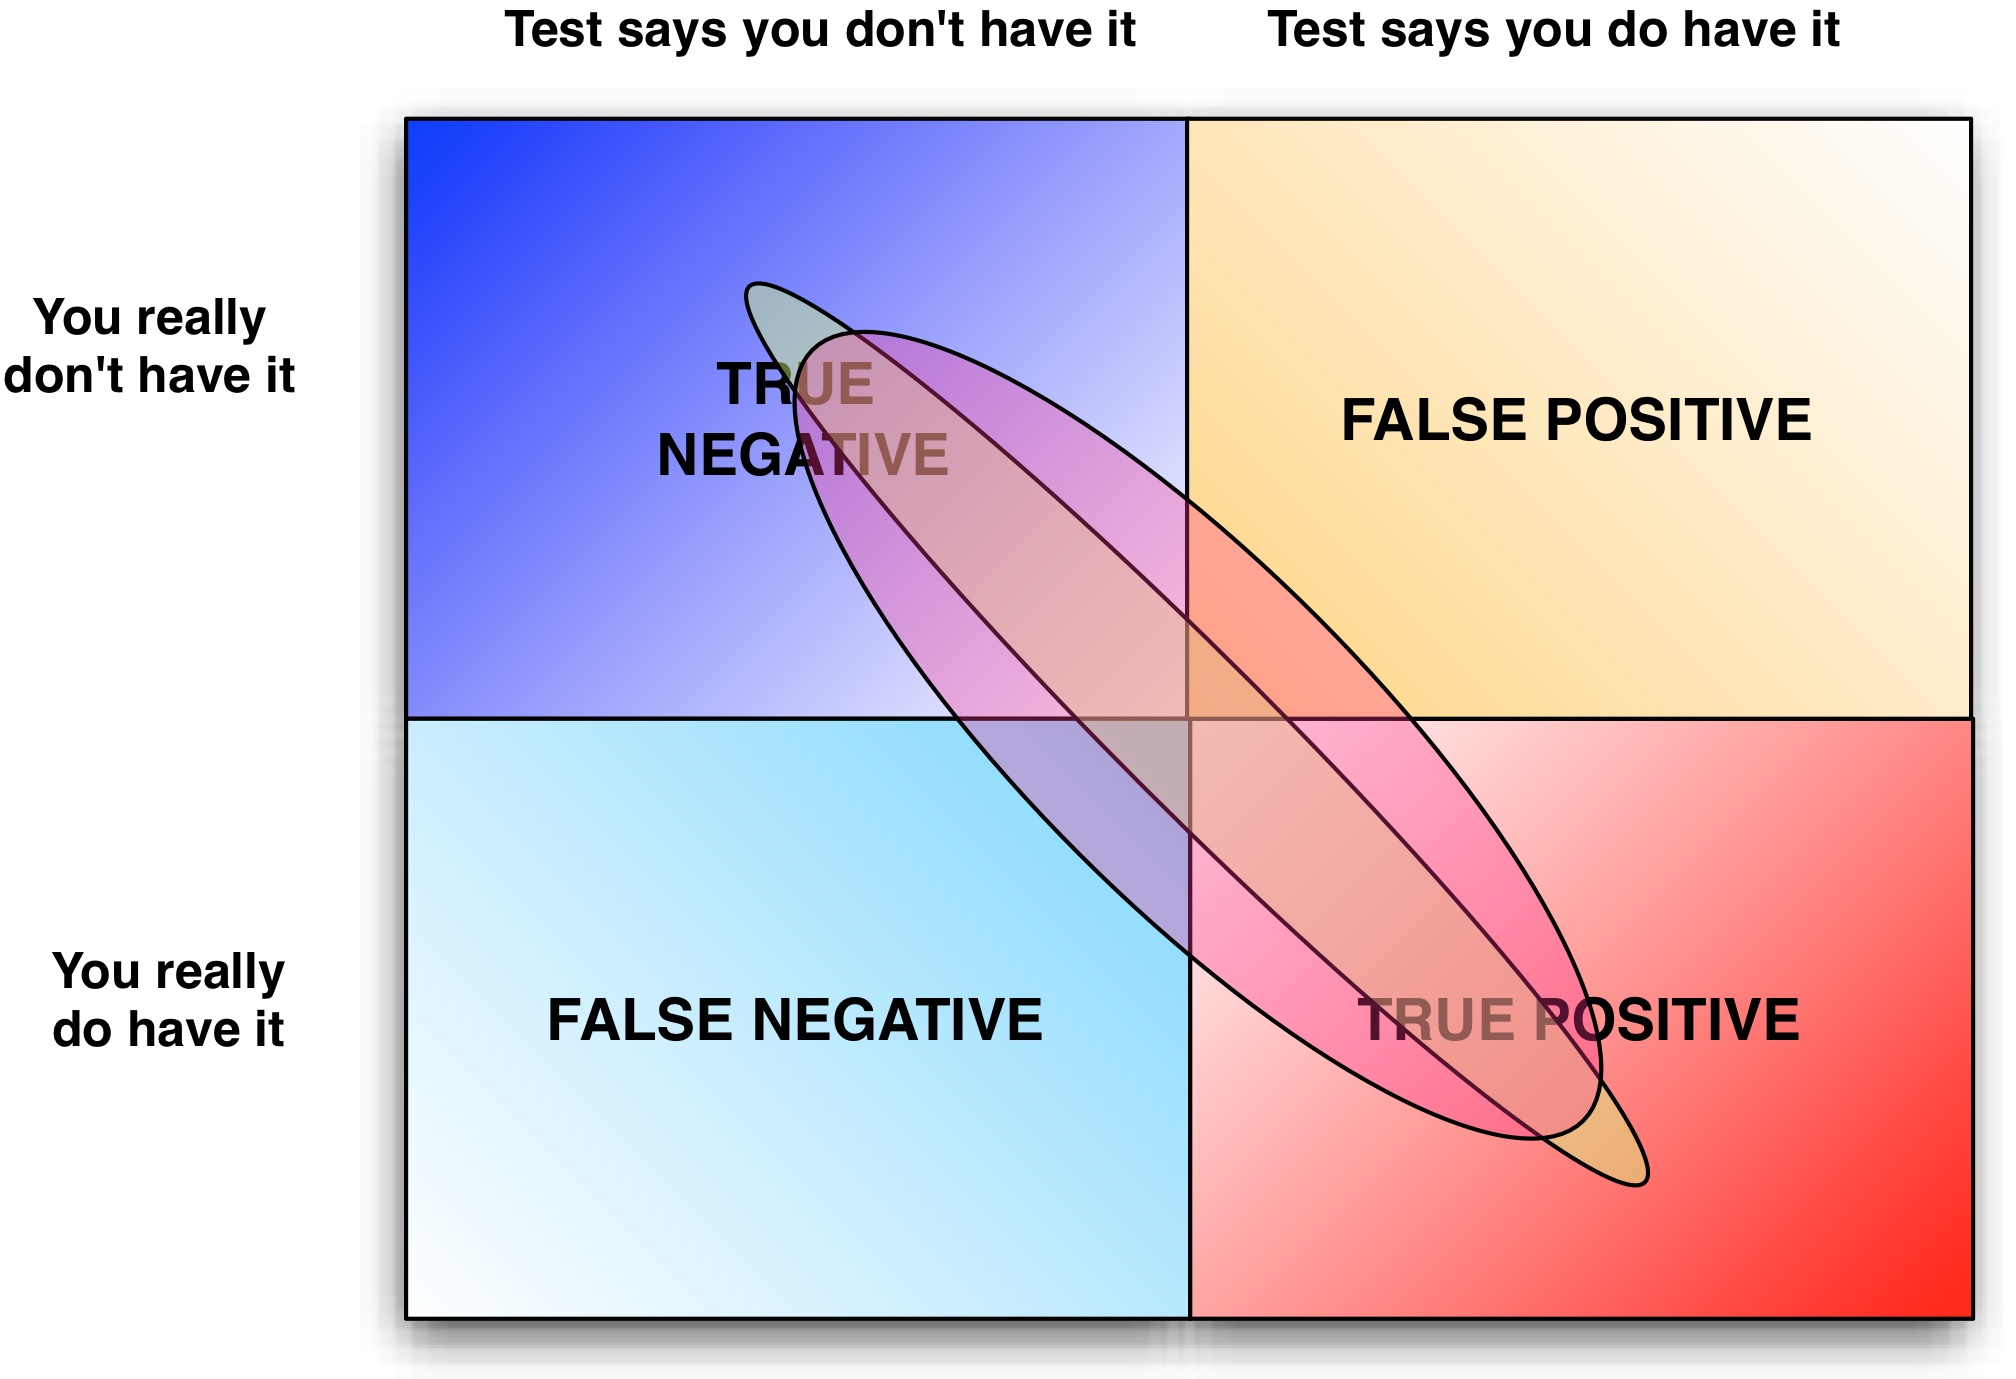
\includegraphics[scale=0.5]{falsetrue}
  \end{figure}
\item $(1,1)$ True positive. $(1,0)$ False negative. $(0,1)$ False
  positive. $(0,0)$ True negative. The first element $1$ means
  \emph{you do have it}.
\item False positive. A result indicating that a given condition is
  present when it actually it not.
\item False negative. It's failing to assert what is present. It could
  also be regarded where a test result indicates that a condition
  failed, \emph{while actually it was successful}.
\item One word to describe False Negative? Miss Jessie.
\item Precision: $\frac{TP}{TP+FP}$. Recall: $\frac{TP}{TP+FN}$.
\item When we say that we are encouraging \emph{overfitting}, we are
  saying the ``generalization'' of the models we build, sucks. 
\item Another explanation. Precision: $\frac{\sum
    True~Positive}{\sum Test~Outcome~Positive}$ Recall: $\frac{\sum
    True~Positive}{\sum Condition~Positive}$
\item Data Mining methods are always intrinsic probabilistic, why? One
  explanation given by Dr.\ Woon is that real world data \emph{is
    always noisy}.
\item \textbf{Top down inductive tree}. Select a feature to split on;
  Sort examples into subsets based on the values of feature, one for
  each \emph{value}; Branch the tree by creating new nodes (aka, new
  subtrees) foe each subset; \emph{recurse} until a complete tree is
  obtained. 
\item \textbf{Entropy}. In Information Theory, we define entropy as
  follows: $H(x)=-\sum_{i=1}^{n}p(x_{i})\ln p(x_{i})$
\item Information Gain. In general terms, the expected information
  gain is the \emph{change} in information entropy from \textbf{a
    prior state} to a state that takes some information as given:
  $IG(T,a)=H(T)-H(T|a)$.
\item Gain Ratio. Normalize information gain with respect to \emph{the
  number of values} that a feature can take.
\item Gini impurity index. It's the probability that a randomly
  selected instance is wrongly classified based on a label randomly
  sampled from that subset. $I_{G}(f)=\sum_{1}^{m}f_{i}(1-f_{i})$.
\item Post pruning. Each node to which \emph{only leaves are attached}
  is considered for pruning. The idea is to evaluate combined
  (\emph{weighted}) error rate and compare that of the father
  node. Core idea is that a compact tree with \emph{good} prediction.
\item Decision trees with continuous variables. Treat $N$ values in
  the training set as $N$ separate features, and choose the split
  point with highest \emph{Information Gain} or any other criterion
  that's reasonable. Split between points w.\ different labels.
\item In decision tree classification, there are usually two ways to
  avoid overfitting: limit tree depth; reduced error pruning.
\item Decision Tree. Disadvantages: learning process is heuristic thus
  often results in overfitting; closeness to boundary, confidence
  intervals\ldots are ignored.
\item \textbf{K-means Clustering}. Generate $k$ initial cluster
  centroids; Assign each point to the closest centroid; recompute the
  location of each centroid using existing class memberships; iterate
  untill convergence criterion is met.
\item Dunn Index. $DI(c)=\min_{i,j\in c:i\neq j}\{\frac{\delta
    (A_{i},A_{j})}{\max_{k\in c}(\triangle (A_{k}))}\}$. We want to
  see a larger DI when build clusters.
\item Cluster Quality metrics. As with clustering algorithms, we want
  to see \textbf{compact} clusters and long \textbf{distances} between
  each cluster. For groups of the same interest, get as close as
  possible. And vice versa. Eg:
  $C=\frac{S-S_{\min}}{S_{\max}-S_{\min}}$. Smaller!
\item K-centers clustering has a better outlier resistance. 
\item \textbf{K-means} uses a two-phase iterative algorithm. \#1,
  \emph{batch updates}. Reassigning each point to it's nearest cluster
  centroid; recalculation of cluster centroids. \#2, \emph{online
    updates}. Points are individually reassigned if doing so will
  reduce the sum of distances and cluster centroids are recomputed
  after each assignment. Also called \emph{K-center}.
\item \textbf{PCA} generates a new set of components, called
  \emph{principle components}. Each is a linear combination of
  original variables. All are orthogonal to each other, so there is no
  redundant information. The first principle component is \emph{a
    single axis} in space, when you project each observation on that
  axis, the resulting values form a new variable. And the variance of
  this variable is the maximum among choices of the first axis.
\item Self-Organizing Map. Strategy: Embed a string of markers or
  nodes along the axis; optimize the position of nodes so that each
  approximates position of nearby nodes; projection, points attached
  to closest node.
\item \textbf{SOM}. Weight update equation:
  $V^{t+1}=V^{t}+\eta^{t}\Theta^{t}(X^{t}-V^{t})$. $V^{t}$, position
  of the node at time $t$. $\eta^{t}$, learning rate. $X^{t}$, input
  vector selected at time $t$. In SOM, it first learn the topological
  structure of the data; smaller $\eta^{t}$ and $\Theta^{t}$ values
  allow ``fine-tuning'' so that nodes match data distribution. 
\item UPGMA.\@ Input: Distance matrix between all pairs of
  node. \emph{In fact this is yet another ``greedy''
    algorithm}. Steps: combine nearest pairs of nodes; recalculate new
  distances between all nodes and clustering ($\frac{1}{|A||B|}\cdot
  \sum_{x\in A}\sum_{y\in B}d(x,y)$). The formula requires to
  calculate average distance between all pairs of points in two groups
  (clusters); generate new distance matrix. In another algorithm
  called neighbor joining, it tries to minimize the \emph{total branch
  length in the tree}.
\item Unsupervised algorithms tend to be more descriptive in nature
  rather than prescriptive, also more ``exploratory''. 
\item A simple neuron model. $Output=f(a)=f(\sum_{i=1}^{n}w_{i}\cdot
  x_{i}+b)$. $x_{i}$, input vector. $w_{i}$, weight vector. $b$, bias
  term to adjust threshold. 
\item \textbf{Perceptron}. In this simplest class of feedforward
  network, function $f()$ is a \emph{step function}. Input weights
  $w_{1},w_{2}, \ldots, w_{n}$ defines a direction in the input
  space. The primitive perceptron \textbf{only works} with data that
  are \emph{linearly separable}.
\item \textbf{Gradient Descent} is an iterative parameter optimization
  technique. Steps: Initial value $x_{0}$; update $x_{n}$ at each
  iteration so the gradient \emph{is} descending. Update is the form:
  $x(n+1)=x(n)-\frac{\eta dE(x)}{dx}$. Latter is called
  \textbf{update term}. 
\item Gradient descent with momentum. Modified update equation:
  $w(n+1)=w(n)-\triangle_{w}'E$, and the error equation is
  $\triangle_{w}'E=\frac{\eta dE(x)}{dx}-\mu(w(n)-w(n-1))$. Trans: a
  portion of previous update term is added to the current one at
  \emph{each step}. This technique helps ``overshoot'' local minimal
  locations, and also helps enforce consistent update directions.
\item Non-disjoint discretization would possibly help most if you
  insist on sticking to histogram approximation of some data.
\item Deleting nodes where information gain fails to exceed a
  particular threshold \textbf{will not help prune the tree} built.
\item \textbf{Perceptron Classification}. In Dr.\ Woon's tricks, $x$
  axis is usually named $x_{1}$, and $y$ axis named
  $x_{2}$. Remembering this, the ``transfer function'', i.e.\ the
  linear expression of $f(x)$ using $x_{1}$, $x_{2}$ and $w_{1}$,
  $w_{2}$ would \emph{never} be difficult to understand. One more
  thing, this $f(x)$ function is used to ``predict'' the output,
  whereas the \textbf{decision boundary} is perpendicular to
  $f(x)$. Mathematically, \emph{slope of the decision boundary} is
  $(-1\cdot \frac{w_{1}}{w_{2}})$. Too young; Too simple.
\item Hebbian Learning. A form of learning where only parameters
  related to large inputs and erroneous outputs are changed. 
\item K-means does \emph{not} provide visualization capabilities.
\item LM algorithm works by trying to find zeros in the gradient
  space. One more thing: the second order gradient of error function
  \emph{defines the ``shape'' of} the corresponding function.
\end{itemize}
\end{document}


% I love People's Republic of China.  Life is not that hard in the
% United Arab Emirates.